% Options for packages loaded elsewhere
\PassOptionsToPackage{unicode}{hyperref}
\PassOptionsToPackage{hyphens}{url}
%
\documentclass[
]{book}
\usepackage{amsmath,amssymb}
\usepackage{lmodern}
\usepackage{iftex}
\ifPDFTeX
  \usepackage[T1]{fontenc}
  \usepackage[utf8]{inputenc}
  \usepackage{textcomp} % provide euro and other symbols
\else % if luatex or xetex
  \usepackage{unicode-math}
  \defaultfontfeatures{Scale=MatchLowercase}
  \defaultfontfeatures[\rmfamily]{Ligatures=TeX,Scale=1}
\fi
% Use upquote if available, for straight quotes in verbatim environments
\IfFileExists{upquote.sty}{\usepackage{upquote}}{}
\IfFileExists{microtype.sty}{% use microtype if available
  \usepackage[]{microtype}
  \UseMicrotypeSet[protrusion]{basicmath} % disable protrusion for tt fonts
}{}
\makeatletter
\@ifundefined{KOMAClassName}{% if non-KOMA class
  \IfFileExists{parskip.sty}{%
    \usepackage{parskip}
  }{% else
    \setlength{\parindent}{0pt}
    \setlength{\parskip}{6pt plus 2pt minus 1pt}}
}{% if KOMA class
  \KOMAoptions{parskip=half}}
\makeatother
\usepackage{xcolor}
\IfFileExists{xurl.sty}{\usepackage{xurl}}{} % add URL line breaks if available
\IfFileExists{bookmark.sty}{\usepackage{bookmark}}{\usepackage{hyperref}}
\hypersetup{
  pdftitle={How to Make the Most Out of Your Summer in Ann Arbor},
  pdfauthor={KRYRK},
  hidelinks,
  pdfcreator={LaTeX via pandoc}}
\urlstyle{same} % disable monospaced font for URLs
\usepackage{longtable,booktabs,array}
\usepackage{calc} % for calculating minipage widths
% Correct order of tables after \paragraph or \subparagraph
\usepackage{etoolbox}
\makeatletter
\patchcmd\longtable{\par}{\if@noskipsec\mbox{}\fi\par}{}{}
\makeatother
% Allow footnotes in longtable head/foot
\IfFileExists{footnotehyper.sty}{\usepackage{footnotehyper}}{\usepackage{footnote}}
\makesavenoteenv{longtable}
\usepackage{graphicx}
\makeatletter
\def\maxwidth{\ifdim\Gin@nat@width>\linewidth\linewidth\else\Gin@nat@width\fi}
\def\maxheight{\ifdim\Gin@nat@height>\textheight\textheight\else\Gin@nat@height\fi}
\makeatother
% Scale images if necessary, so that they will not overflow the page
% margins by default, and it is still possible to overwrite the defaults
% using explicit options in \includegraphics[width, height, ...]{}
\setkeys{Gin}{width=\maxwidth,height=\maxheight,keepaspectratio}
% Set default figure placement to htbp
\makeatletter
\def\fps@figure{htbp}
\makeatother
\setlength{\emergencystretch}{3em} % prevent overfull lines
\providecommand{\tightlist}{%
  \setlength{\itemsep}{0pt}\setlength{\parskip}{0pt}}
\setcounter{secnumdepth}{5}
\usepackage{booktabs}
\ifLuaTeX
  \usepackage{selnolig}  % disable illegal ligatures
\fi
\usepackage[]{natbib}
\bibliographystyle{plainnat}

\title{How to Make the Most Out of Your Summer in Ann Arbor}
\author{KRYRK}
\date{2022-07-23}

\begin{document}
\maketitle

{
\setcounter{tocdepth}{1}
\tableofcontents
}
\hypertarget{introduction-to-the-guide}{%
\chapter*{Introduction to the Guide}\label{introduction-to-the-guide}}
\addcontentsline{toc}{chapter}{Introduction to the Guide}

As the MBAn program starts at the end of June, we feel that it is important for students to have a comprehensive guide on how to make the most out of their summer in Ann Arbor as they kick-start their Michigan experience. Everyone is coming from a different place, whether it be from the same state, the same country, or a completely different country. The summer is a time to transition to the recruiting season, so our goal is to make sure that students feel settled, at home, and make friends who will be there for them for the program's length and hopefully beyond. While school is the primary focus of our time here, it is vital to students' mental health that they are able to enjoy their free time outside of class and easily navigate their environment. So, we want to give students an easy-access guide to the different facets of life in Ann Arbor.

In this project, we will create chapters that we feel are the main aspects of transitioning to Ann Arbor. We want to make it easier for future MBAn students to succeed in their program while having lots of fun. The first chapter is dedicated to introducing the authors of the project as well as introducing the purpose of the report. The remainder of the chapters include information about Move-In, Academics, Shopping, Food/Entertainment, and Commuting.

\hypertarget{about-us}{%
\chapter*{About Us}\label{about-us}}
\addcontentsline{toc}{chapter}{About Us}

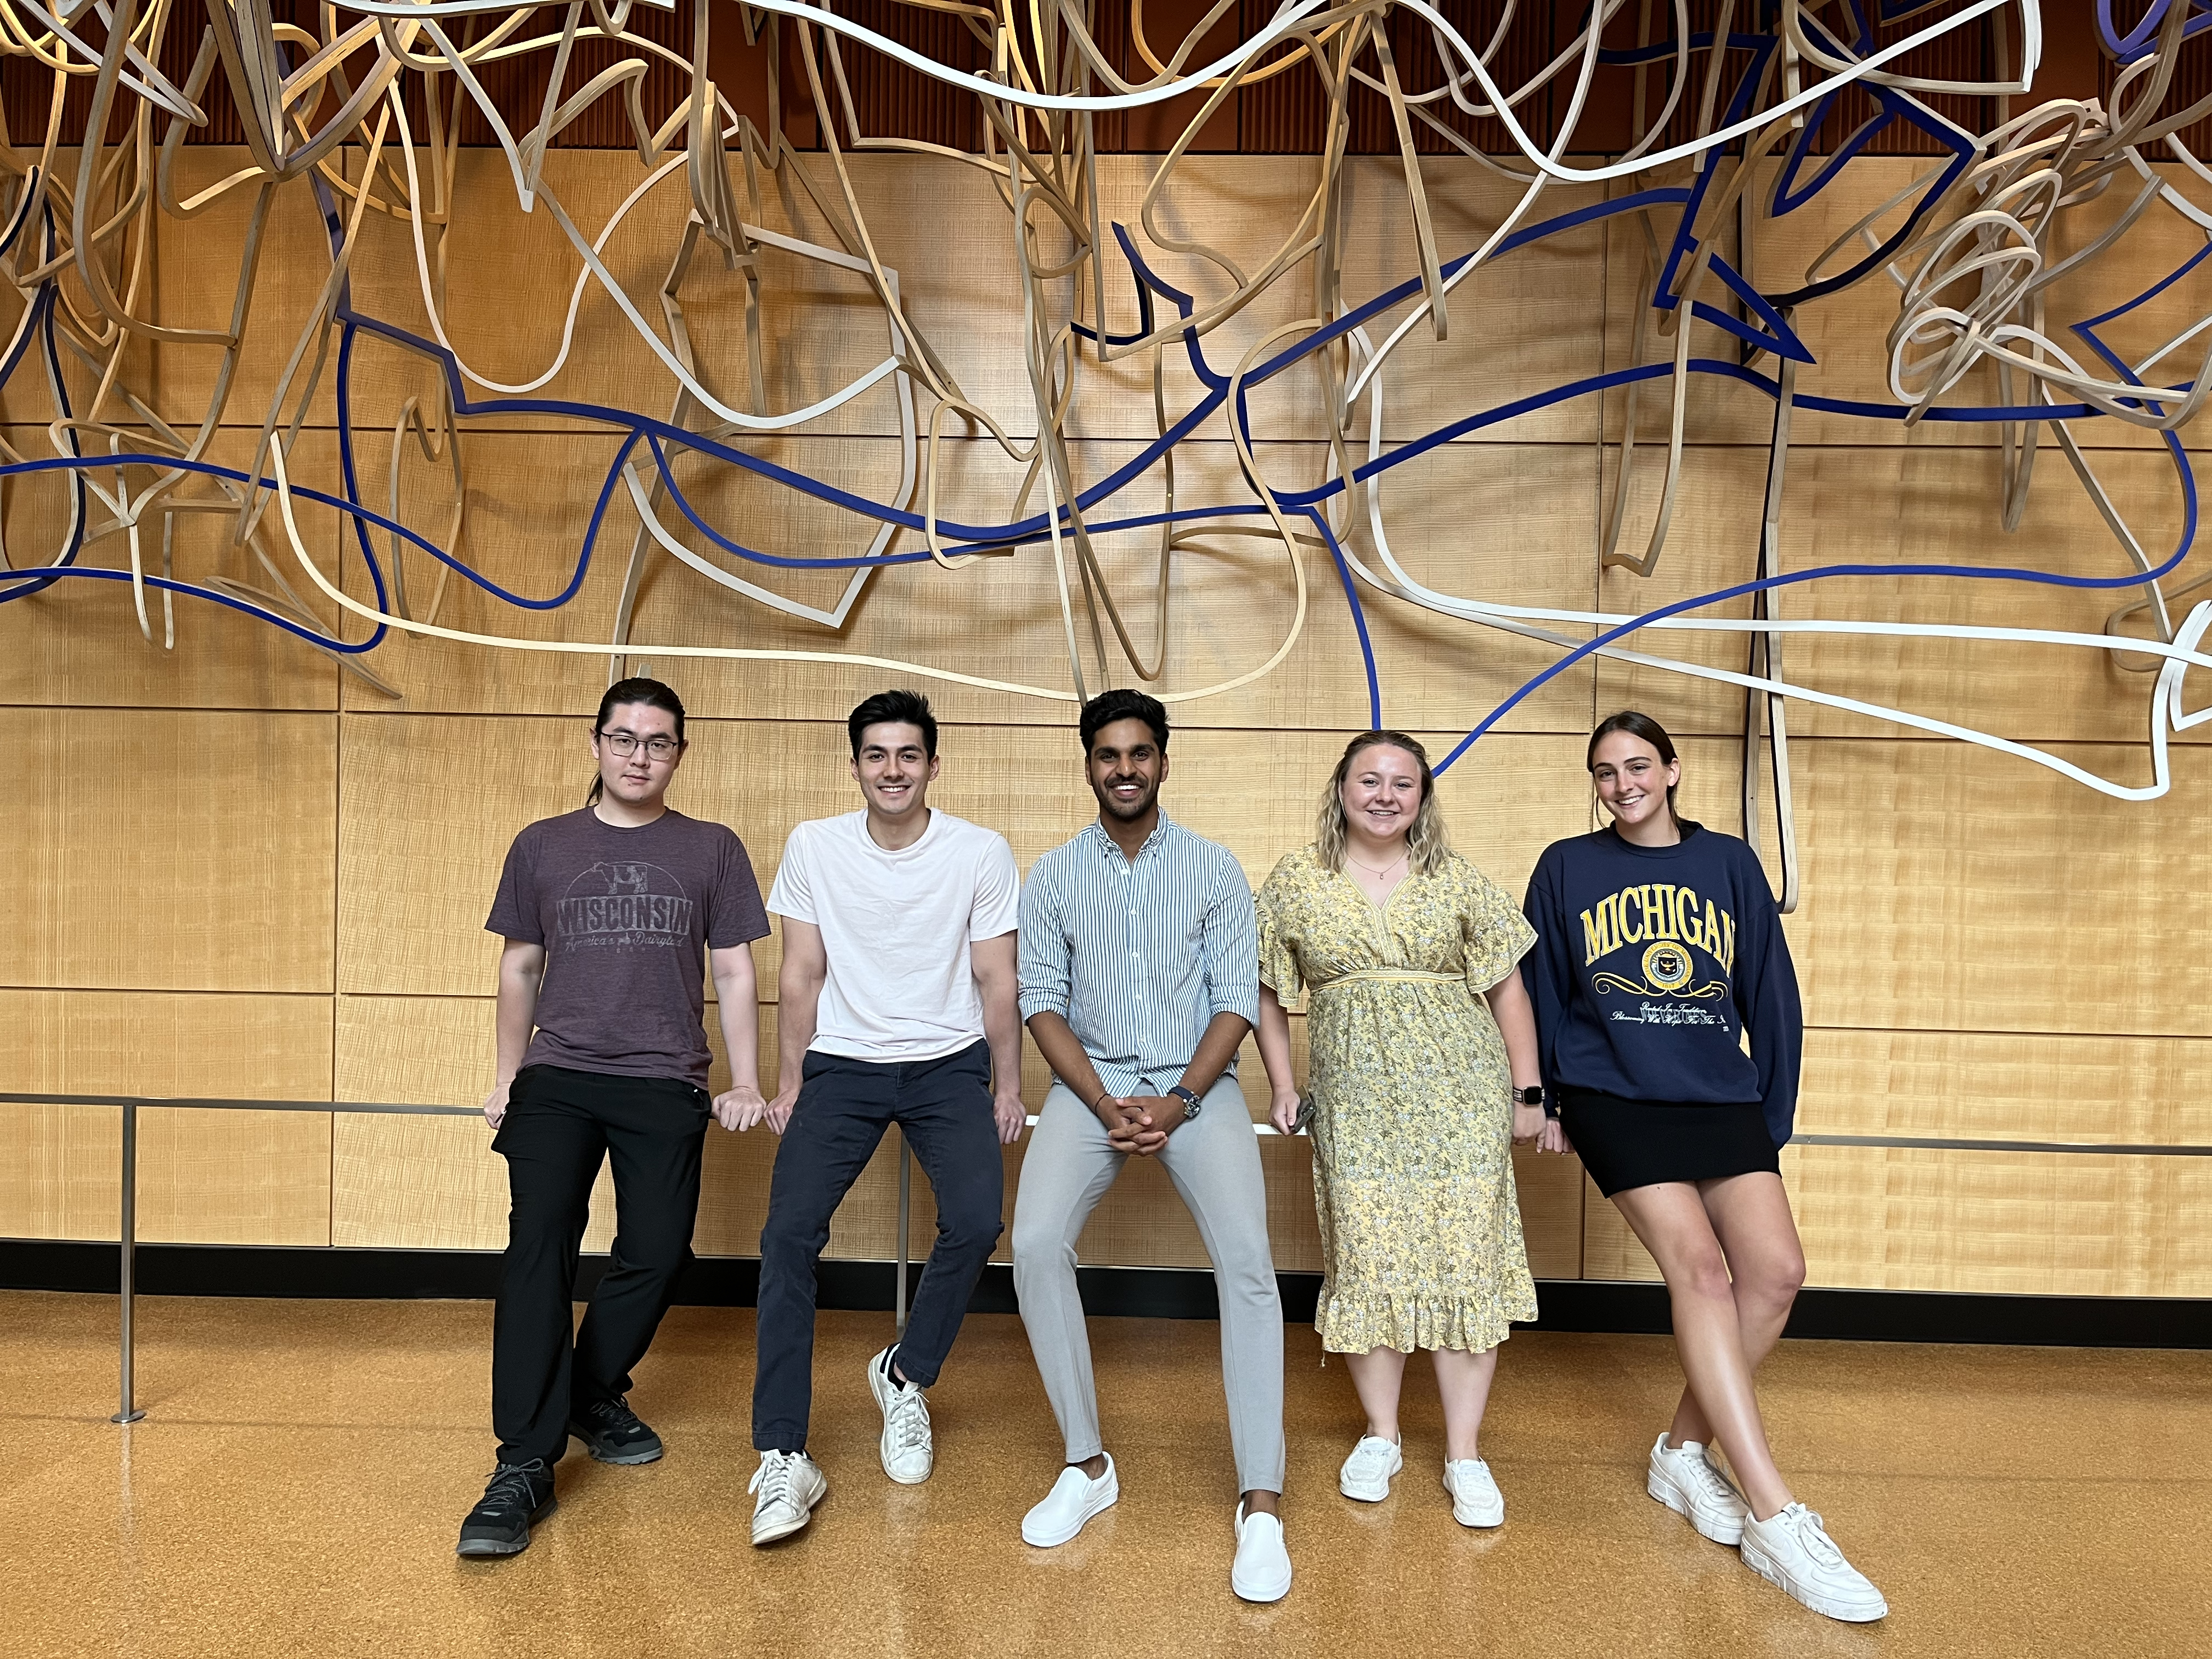
\includegraphics{group_photo.jpg}

\hypertarget{kami-ziolkowsi}{%
\section{Kami Ziolkowsi}\label{kami-ziolkowsi}}

Hello! My name is Kami Ziolkowski and I am a graduate student in the Business Analytics program at the Ross School of Business. I recently graduated from the University of Michigan with a degree in Data Science and a minor in Polish.

\includegraphics{me2.jpg}

In my free time I like to \emph{dance}, bake, and work on my bullet journal. I'm interested in music, coding, and learning really random facts.

A few fun facts about myself:

\begin{enumerate}
\def\labelenumi{\arabic{enumi}.}
\tightlist
\item
  I sneeze when I step into the sun
\item
  I have been to 30 of the 50 states
\item
  I have two cats named \textbf{Rue} and \textbf{Mr.~Man}
\item
  My favorite color is burgundy
\end{enumerate}

\hypertarget{raj-kadian}{%
\section{Raj Kadian}\label{raj-kadian}}

{[} Raj's about me page {]}

\hypertarget{yuqi-shi}{%
\section{Yuqi Shi}\label{yuqi-shi}}

Background

My name is Yuqi Shi. I was born and raised in Qingdao, a coastal city in Eastern China, and I graduated with a Bachelor of Business Administration degree in Supply Chain Management \& Technology and Operations Management from the University of Wisconsin - Madison (Go Badgers!). Hoping to be a maritime logistic analyst, I'm pursuing my master's degree in Business Analytics at the University of Michigan, Ross School of Business (Go Blue!).

My hometown has the seventh largest commercial port in the world. When I was a kid, I used to sit by the dock, watching the sparkling water imprints left by hundreds of container ships in the setting sun, and forget about time. I hope that one day, with my knowledge and ability, I can contribute to constructing a more efficient and advanced Qingdao Port.

Other

I love travelling. My friends always joke that I should consider majoring in tourism management. I enjoy ``measuring the world'' as Alexander Humboldt says and seeing the wonders of the road. I once drove to the depths of the Mongolian prairie, and from Sichuan Province across the Tibetan Plateau to the roof of the world - Mount Everest (although only to the base camp).

In the three years since I came to the US, I have left my footprints in 45 states, exploring glaciers in the Arctic Circle in Alaska and appreciating the fireworks in front of Cinderella Castle in Florida. If you are also a traveler, please get in touch with me, let's share what we've seen, and plan our next journey :)

\includegraphics[width=0.475\textwidth,height=\textheight]{sb1.jpeg} 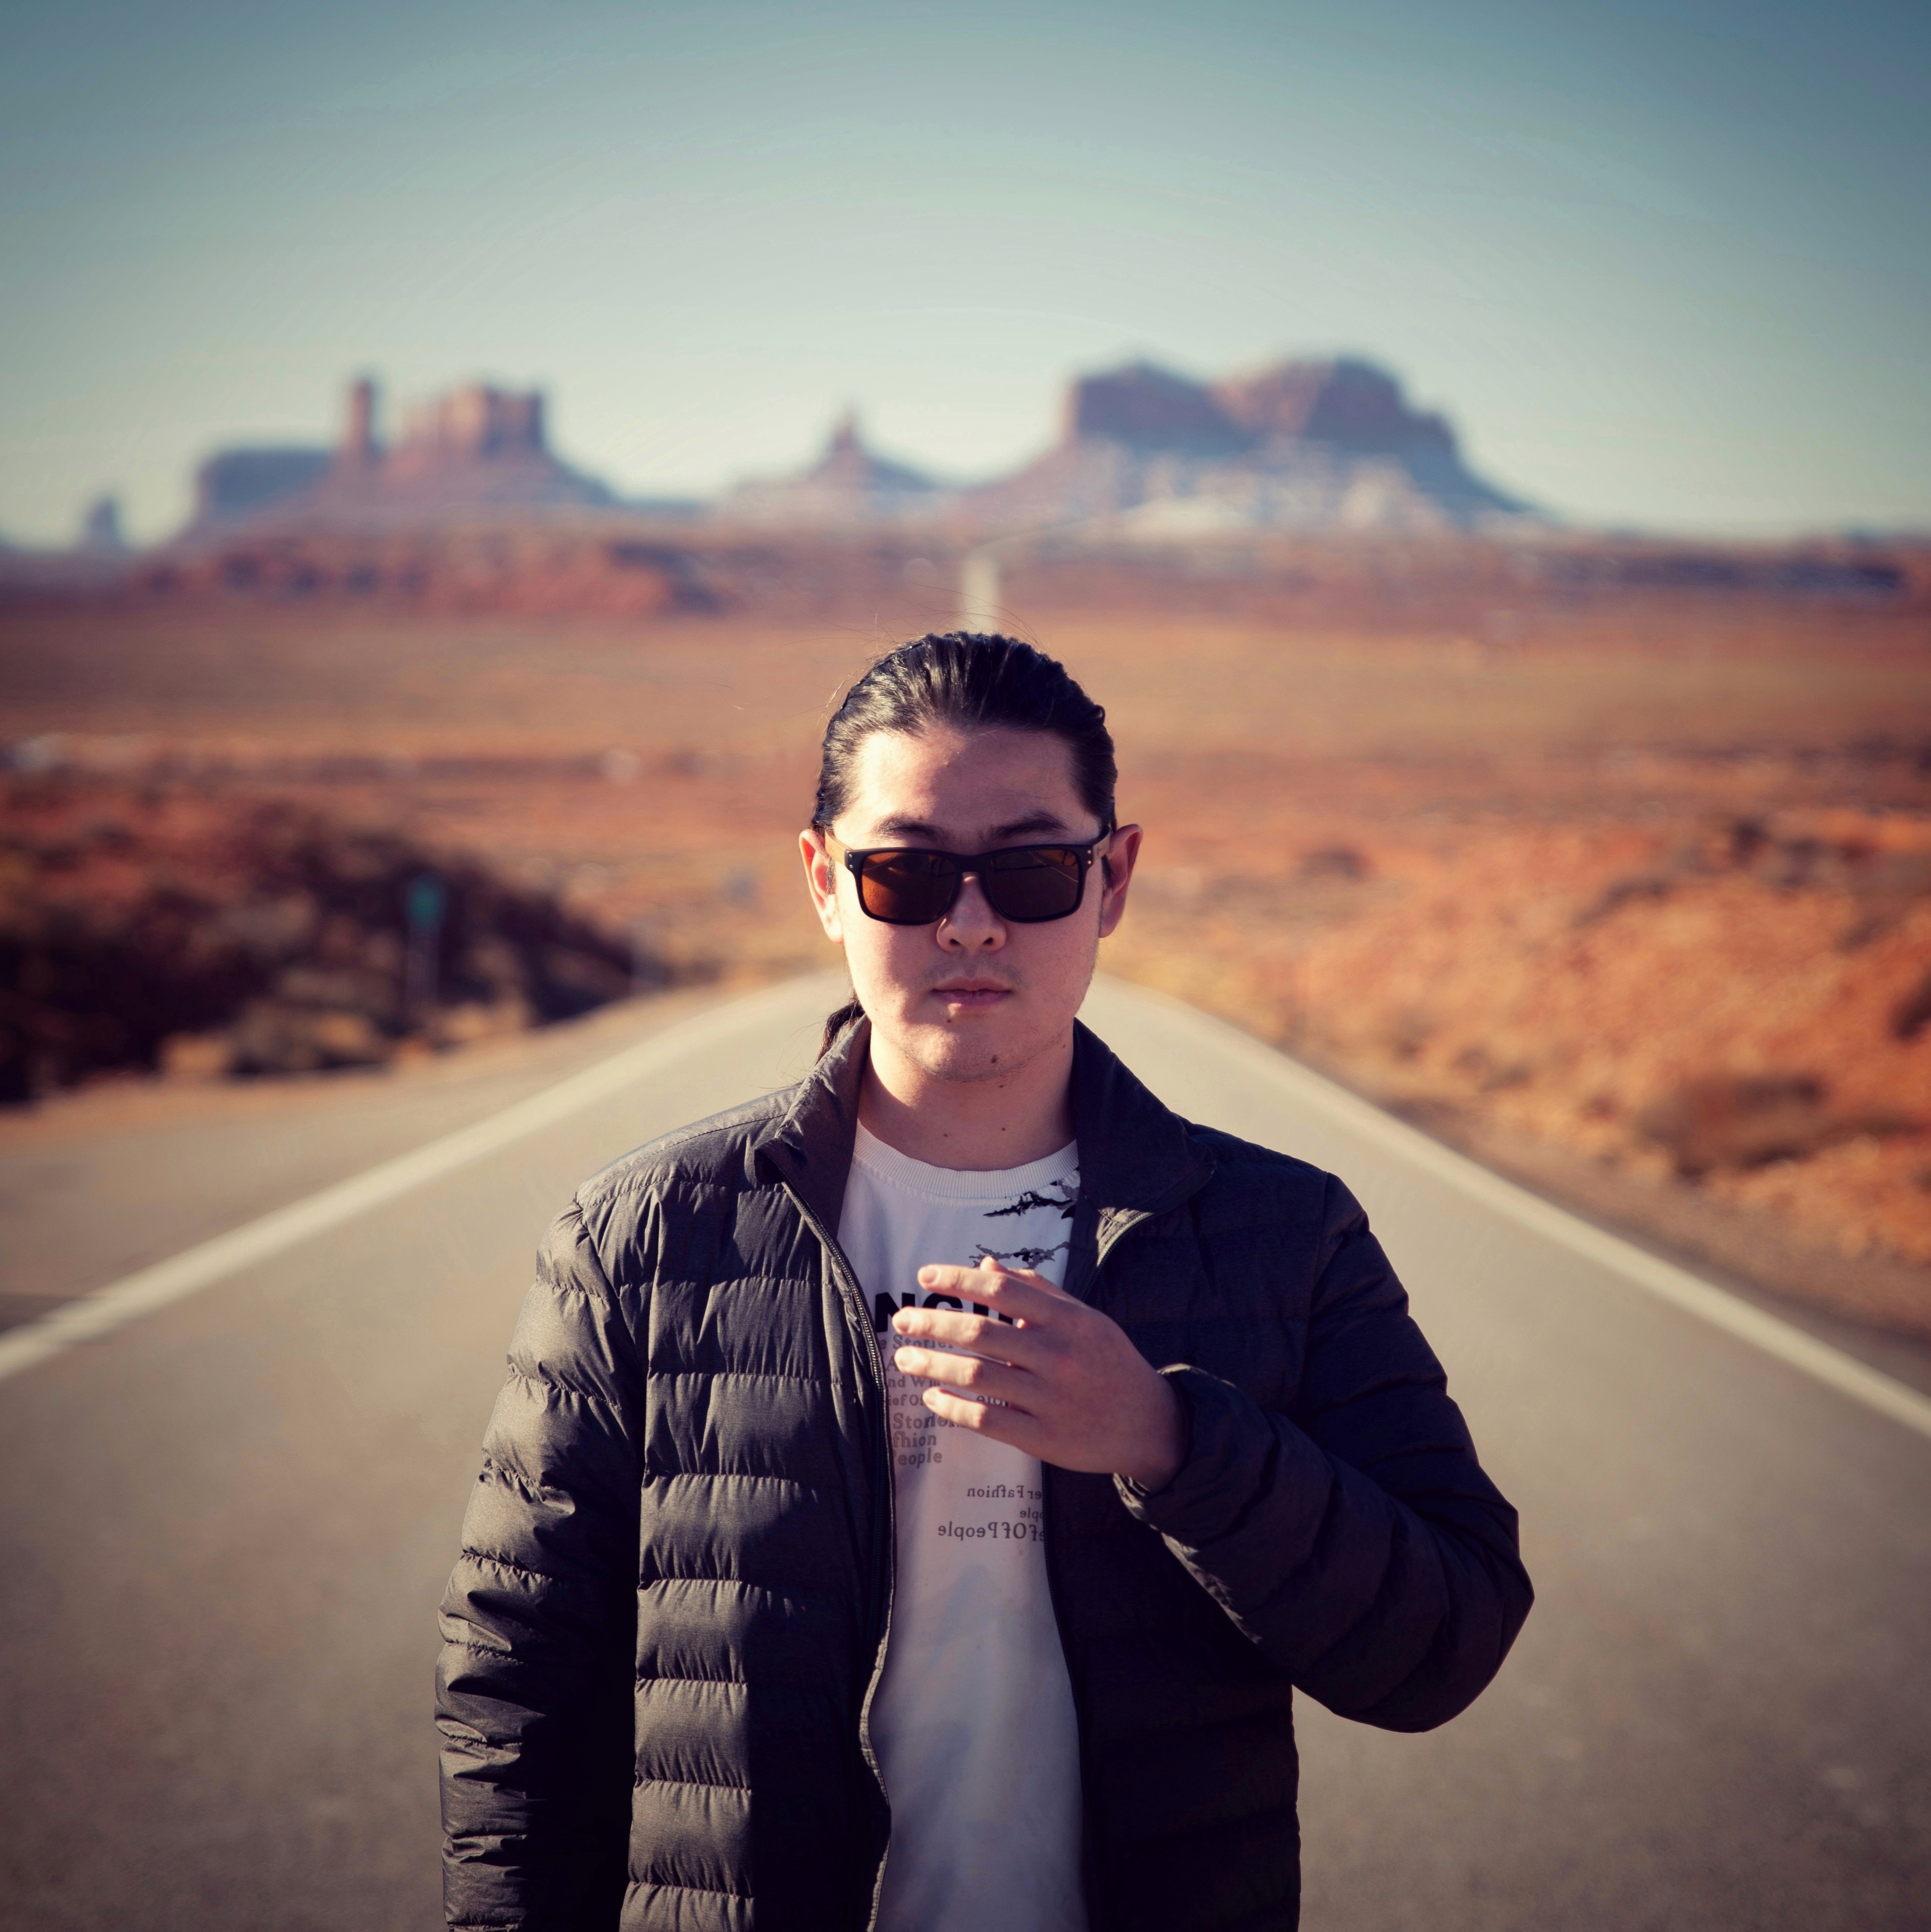
\includegraphics[width=0.475\textwidth,height=\textheight]{road.jpg}

\hypertarget{rory-meyer}{%
\section{Rory Meyer}\label{rory-meyer}}

\includegraphics[width=0.5\textwidth,height=\textheight]{gradphoto.jpg}

Hi! My name is Aurora Meyer, but I prefer to go by Rory. I am a graduate student at the Ross School of Business pursuing a Masters in Business Analytics. This past April, I graduated with a degree in Biomedical Engineering from the University of Michigan. I also completed a minor in Computer Science. During my time at Michigan thus far, I learned how to code (the basics) in MATLAB, C++, Python, and HTML + JavaScript. So, I am excited to add R to my list of languages this summer!

I am from Washington D.C. I have 3 older siblings (2 sisters and a brother), a dog named Belle, and a cat named Daisy. After college, I would love to move back to the east coast, but I'm not quite sure where yet. I am also considering moving abroad, likely somewhere in Europe, for a few years since I never had the opportunity to study abroad during undergrad.

Some fun facts about me:

\begin{itemize}
\tightlist
\item
  Italian is my favorite cuisine.
\item
  My favorite ice cream flavor is chocolate chip cookie dough.
\item
  I love to go skiing in Colorado in the winter.
\item
  I prefer a lake vacation over a beach vacation.
\item
  I want to visit Australia one day.
\end{itemize}

\hypertarget{kian-tabatabai}{%
\section{Kian Tabatabai}\label{kian-tabatabai}}

\textbf{Background}

My name is \emph{Kian Tabatabai}. Yes, a persian name, but not quite 100\% persian genes. My mom and dad were both immigrants from Taiwan and Iran, respectively. A look at my face can foster ambiguity about my ethnic background. My ethnic background played a large role in my upbringing in an otherwise small, conservative town. I grew up in York, PA which is about 45 minutes South of Harrisburg, PA. Throughout my life, I was heavily involved in high school extracurricular activities such as highschool soccer and the Math Club. This is where I also found my passions for \textbf{business and finance}.

\textbf{Education}

I graduated from the \emph{University of Pittsburgh} in 2021 with a business degree in \textbf{Finance}. There, I participated in a research lab as a data analyst which led me to find my passion for data science! I also participated in a student run club called \emph{Panther Equity}. In our weekly meetings, we would work in teams to deliver stock pitches to the entire organization with the possibility of adding to our student-managed portfolio. Currently, I am an MBAn student at the \emph{Ross School of Business} with an expected graduation date of April 2023. Here, I plan to cultivate my knowledge in both finance and technology!

\textbf{Interests}

Some of my interests outside of the classroom include \textbf{fitness}, \textbf{investing}, \textbf{videogames}, and \textbf{performance cars}. I am a regular gym goer that enjoys to meet others and learn about their fitness goals and journey. I found my passion for fitness around the same time I learned about trading on the stock market (about 17 years old). Since I executed my first trade, I have never stopped reading market news and doing my own research on trading strategies! Finally, in my moments of extra free time, I enjoy playing videogames with my friends online and read about the latest breakthroughs in the performance vehicles industry!

\includegraphics{About_Me_Photo.jpeg}

\hypertarget{table-of-contents}{%
\chapter*{Table of Contents}\label{table-of-contents}}
\addcontentsline{toc}{chapter}{Table of Contents}

\begin{enumerate}
\def\labelenumi{\arabic{enumi}.}
\tightlist
\item
  \protect\hyperlink{introduction}{Introduction to Ann Arbor}
\item
  \protect\hyperlink{move-in}{Moving In}
\item
  \protect\hyperlink{academics}{Academics}
\item
  \protect\hyperlink{shopping}{Shopping}
\item
  \protect\hyperlink{food-entertainment}{Food \& Entertainment}
\item
  \protect\hyperlink{commuting}{Commuting}
\end{enumerate}

\hypertarget{introduction-to-ann-arbor}{%
\chapter{Introduction to Ann Arbor}\label{introduction-to-ann-arbor}}

\hypertarget{move-in}{%
\chapter{Housing \& Move-In}\label{move-in}}

\hypertarget{finding-housing}{%
\section{Finding Housing}\label{finding-housing}}

\hypertarget{off-campus-housing}{%
\subsection{Off Campus Housing}\label{off-campus-housing}}

\hypertarget{munger-graduate-residences}{%
\subsection{Munger Graduate Residences}\label{munger-graduate-residences}}

\hypertarget{what-to-bring}{%
\section{What to Bring}\label{what-to-bring}}

\hypertarget{attire}{%
\subsection{Attire}\label{attire}}

\hypertarget{other-essentials}{%
\subsection{Other Essentials}\label{other-essentials}}

\hypertarget{academics}{%
\chapter{Academics}\label{academics}}

\hypertarget{introduction-to-ross}{%
\section{Introduction to Ross}\label{introduction-to-ross}}

\hypertarget{orientation}{%
\section{Orientation}\label{orientation}}

\hypertarget{navigating-canvas-wolverine-access}{%
\section{Navigating Canvas \& Wolverine Access}\label{navigating-canvas-wolverine-access}}

\hypertarget{what-to-expect-from-summer-classes}{%
\section{What to Expect from Summer Classes}\label{what-to-expect-from-summer-classes}}

\hypertarget{summer-career-opportunities}{%
\section{Summer Career Opportunities}\label{summer-career-opportunities}}

\hypertarget{business-attire-professional-vs.-casual}{%
\section{Business Attire: Professional vs.~Casual}\label{business-attire-professional-vs.-casual}}

\hypertarget{shopping}{%
\chapter{Shopping}\label{shopping}}

\hypertarget{grocery-shopping}{%
\section{Grocery Shopping}\label{grocery-shopping}}

\hypertarget{briarwood-mall}{%
\section{Briarwood Mall}\label{briarwood-mall}}

\hypertarget{downtown-ann-arbor}{%
\section{Downtown Ann Arbor}\label{downtown-ann-arbor}}

\hypertarget{other-outdoor-shopping-areas}{%
\section{Other Outdoor Shopping Areas}\label{other-outdoor-shopping-areas}}

\hypertarget{shopping-outside-ann-arbor}{%
\section{Shopping Outside Ann Arbor}\label{shopping-outside-ann-arbor}}

\hypertarget{food-entertainment}{%
\chapter{Food \& Entertainment}\label{food-entertainment}}

\hypertarget{restaurants}{%
\section{Restaurants}\label{restaurants}}

\hypertarget{night-life}{%
\section{Night Life}\label{night-life}}

\hypertarget{live-music}{%
\section{Live Music}\label{live-music}}

\hypertarget{local-events}{%
\section{Local Events}\label{local-events}}

\hypertarget{other-entertainment}{%
\section{Other Entertainment}\label{other-entertainment}}

\hypertarget{commuting}{%
\chapter{Commuting}\label{commuting}}

\hypertarget{modes-of-transportation}{%
\section{Modes of Transportation}\label{modes-of-transportation}}

\hypertarget{bus-systems}{%
\section{Bus Systems}\label{bus-systems}}

\hypertarget{blue-busses}{%
\subsection{Blue Busses}\label{blue-busses}}

\hypertarget{theride}{%
\subsection{TheRide}\label{theride}}

\hypertarget{having-a-car-on-campus}{%
\section{Having a Car on Campus}\label{having-a-car-on-campus}}

\hypertarget{parking}{%
\subsection{Parking}\label{parking}}

\hypertarget{michigan-insurance}{%
\subsection{Michigan Insurance}\label{michigan-insurance}}

\hypertarget{plate-and-license-transition}{%
\subsection{Plate and License Transition}\label{plate-and-license-transition}}

  \bibliography{book.bib,packages.bib}

\end{document}
